% Chapter 3

\chapter{Project 2b: Radix sort} % Main chapter title

\label{Chapter3} % Change X to a consecutive number; for referencing this chapter elsewhere, use \ref{ChapterX}

\lhead{Chapter 3. \emph{Radix sort}} % Change X to a consecutive number; this is for the header on each page - perhaps a shortened title

%----------------------------------------------------------------------------------------


\section{Introduction}



\section{Implementations}




\subsection{Counting sort (CS)}
We start by finding the greatest value in the list gKey.
gKey = Max(Array)+1
We use gKey to create a new array C and for every entry in C we set the value to 0.
in line 4-5 we go through the input array and use the Histogram array to keep trak of how many of a specific element we have, so for all the elements in array we go to the equvalent index in Histogram and increase it by 1.
In line 6-7 we use the Histogram to calculate the starting index of each key in array.
In the last loop we go through the Histogram array and we iterate from the last index and down to the beginning of the array.
The index of Histogram[array[j]-1] is where the j'th element of array should be in the result array.
Then we count down the Histogram[array[j]] by 1.
This work for the case where we have multiple of the same key and in the case where we have only one of each key, because in line 11 we decrease the starting index by 1 after having placed one instance of the key, so the previous won't be overwritten.
\lstinputlisting[language=C++, firstline=32, lastline=46, numbers=left]{./Figures/Project2b/CountingSort.cpp}

\subsection{Quick sort (QS)}
We use a Quick Sort from a \verb!C++! library because we want to compare our other algorithms with one that has a running time of $ O(n\cdot \log n) $ which Quick Sort does.
We call the library function in line 1 which takes an array, the size of the array, the type of elements (int in our case) and a compare function.
\lstinputlisting[language=C++, firstline=20, lastline=21, numbers=left]{./Figures/Project2b/QuickSort.cpp}
The compare function states that the input should e sorted from the smallest key to the greatest.
\lstinputlisting[language=C++, firstline=13, lastline=16, numbers=left]{./Figures/Project2b/QuickSort.cpp}
\subsection{Most significant digit (MSD)}

The MSD radix sort is implemented as follows:
\begin{verbatim}
  // Pass 0
  queue<int> buckets[N_BUCKETS];
  for (int i = 0; i < arrSize; i++) {
    // Add to bucket
    buckets[ sortedArray[i] >> (K-D) ].push(sortedArray[i]);
  }
  // Pass 1 (and the rest, recursively)
  for (int b = 0; b < N_BUCKETS; b++) {
    msdRecursive(buckets[b], 1);
  }
  return sortedArray;
\end{verbatim}


It makes use of the following recursive method:
\begin{verbatim}
void msdRecursive(queue<int> bucket, int pass) {
  if (bucket.empty()) return;
  
  // Base case (this bucket is already fully sorted).
  if (pass == N_PASSES) {
    while(!bucket.empty()) {
      sortedArray[sortArrIdx] = bucket.front();
      bucket.pop();
      sortArrIdx++;
    }
    return;
  }
  // Sort this bucket into some new buckets.
  queue<int> buckets[N_BUCKETS];
  while(!bucket.empty()) {
    const int key = bucket.front();
    bucket.pop();
    // Add to bucket
    buckets[ (key >> (K - (pass+1)*D)) & MASK_D ].push(key);
  }
    // Example (K=8, D=2, pass=1, so we have already sorted by AB, and now we look at CD):
    // (ABCDEFGH >> (8 - (1+1)*2)) & 00000011
    // (ABCDEFGH >> 4) & 00000011
    //  0000ABCD & 00000011
    //  000000CD

  // Now, sort all buckets recursively.
  for (int b = 0; b < N_BUCKETS; b++) {
    msdRecursive(buckets[b], pass+1);
  }
}
\end{verbatim}



\subsection{Least significant digit (LSD)}
To have something to compare the Multi-core Radix Sort to, we implemented, among others, Least Significant Digit (LSD) radix sort. 
The idea is to sort the input array of keys into buckets starting from the lowest significant digit. After each sorting into buckets for a digit an array sorted from the that digit is produced. 
This is done for each digit until the input array is fully sorted. 

The implemtation uses C++ std:queue structure to simulate buckets. We assume that this data structure utilizes memory and computation quite effectively, and it seem logical to use this instead of creating our own bucket data structure.
In the method 'sort' the pgram sorts the array as mentioned before, by iterating over the digits starting from the lowest significant one. At each iteration sorting the keys into buckets and then creating a new array from these buckets.
\begin{lstlisting}[numbers=left]
...
for (int i = 0; i < N_PASSES; i++) {
  for (int j = 0; j < arrSize; j++) {
    // Add to bucket
    buckets[ (sortedArray[j] >> (K-i*D)) & MASK_D ].push(sortedArray[j]);
  }
  // Create sorted array from buckets
  int sortArrIdx = 0;
  for (int k = 0; k < N_BUCKETS; k++) {
    while(!buckets[k].empty()) {
      sortedArray[sortArrIdx] = buckets[k].front();
      buckets[k].pop();
      sortArrIdx++;
    }
  }
}
\end{lstlisting}
\verb!sortedArray[j] >> (K-i*D)) & MASK_D! gets the digit we want to look at by right shifting the value and anding it with a bit mask containing 0s except for the lowest D bits, which is 1s.

The algorithm was straight forward to implement an contains no complex computation. If one wanted to improve performance a differen datastructure for buckets could maybe be used.


\subsection{MSD - using arrays (MSD\_arr)}


\subsection{LSD - using arrays (LSD\_arr)}
This version has not been implemented, but it could be done by making similar modifications to LSD as above.


\subsection{Multicore radix sort (MCR) \citep{radixSort}}
The implementation of Multi-core Radix Sort (MCR) is based on the approach in \citep{radixSort}. The idea behind is to use the benefits of both MSD and LSD and making the algorithm parallel to decrease computation time. 
The algorithm first partitions the input array into buckets with based on MSD and then sort each of theses buckets locally with using LSD.  
MSD has the disavangtage of not being very effective on arrays of small size or values is close to each other, because it can results of a lot of empty buckets. 
But has the advantage that when the values is sorted by one digit sorting by next digit only moves around the 
LSD on the other hand ...

The implementation is based on the pseudocode from the forementioned article:
\begin{figure}[htbp]
	\centering
		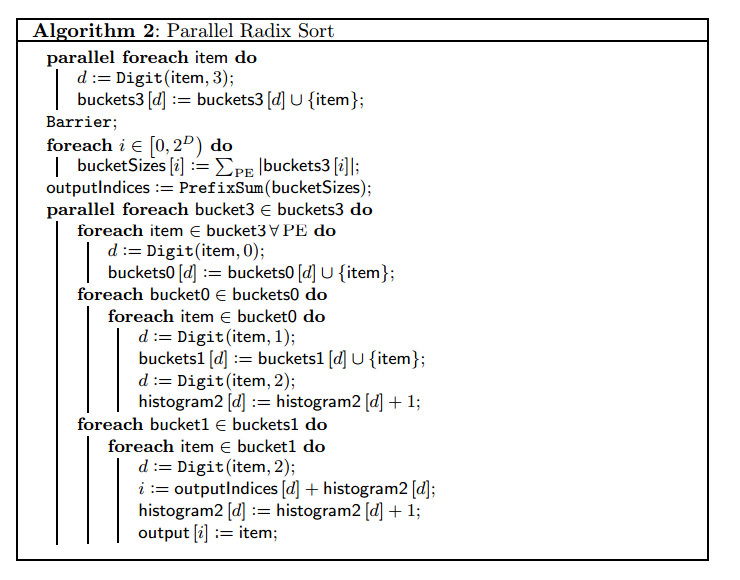
\includegraphics[width=\textwidth]{./Figures/Project2b/MultiCoreRadix_Pseudo.jpg}
		\rule{35em}{0.5pt}
	\caption[Branch misses]{
	Bla bla bla.
	}
	\label{fig:Branch_misses}
\end{figure}
As in the pseudocode the program starts out by sorting the array based on the most significant digit in parallel, then serial compute output indicies (PrefixSum in the pseudocode) and finally parallel sort each bucket based on LSD.  
The parallel parts is implemented using POSIX threads (<pthread.h>), which by default utilizes multicore cpus by starting each thread on a new cpu.

The program has two 2D arrays which respectively holds buckets and bucket histograms for each thread. These are called threadBucketArrays and threadNextArrays.
Each of the bucket arrays in threadBucketArrays inititally took up N x M space, where N is elements in the input array and M is number of buckets.
This means a lot of space had to be reserved by the program. To minimize this space usage, N is bound by the number of elements assigned to the current thread.
This yields that each bucket array takes up (N / P) x M, where P is the number of threads. 

The parallel MSD part (first part) assigns part of the input array to each thread, which then sort the elements int buckets based on the most significant digit.
The sorting is saved in the formentioned shared threadBucketArrays using threadNextArrays to index these bucket arrays:
\begin{lstlisting}
...
bucketArray[ putInBucket*nElemsAssigned[tInfo->threadNum] + nextArray[putInBucket] ] = inputArray[i];
nextArray[putInBucket]++; 
... 
\end{lstlisting}
bucketArray and nextArray coresponds to the threads arrays in threadBucketArrays and threadNextArrays.

The next part consist of the program computing (serial) output indices used to index the output array by traversing over the all the threads nextArrays.   
The array computed from this, ouputMSDStartIndices, is a kind of prefix sum over sizes of the MSD-bucket, but where the values are shifted on to the right in the array (i.e. the first element is 0).

In the last part, the MSD buckets is divided among the threads, which sort the assigned buckets locally based on LSD and then write sorted values to the output array.
For each MSD bucket assigned to a thread, it first sort the values in the bucket into new buckets (locally) based on the lowest significant digit. This is straight forward.
Then traversing through the bucket sorted by lowest significant digit, the values are divided into buckets depending on the second lowest significant digit.
And in same traversal a histogram for the third lowest significant digit is produces.
\begin{lstlisting}
...
  for (int bucket = 0; bucket < nBuckets; bucket++) {
    for (int i = 0; i < nexts0[bucket]; i++) {
      elem = buckets0[bucket*arraySize + i];

      // Put in bucket
      putInBucket = (elem >> shiftRight2nLast) & lsdBitMask;
      buckets1[putInBucket*arraySize + nexts1[putInBucket]] = elem;
      nexts1[putInBucket]++;

      // Histogram
      histIdx = (elem >> shiftRightLast) & lsdBitMask;
      histogram2[histIdx]++;
    }
  }
...
\end{lstlisting}
This histogram is then used to produce a prefix sum following same procedure as for the output indices.
\begin{lstlisting}
... 
  prefixSum2[0] = 0;
    for (int i = 0; i < nBuckets; i++) {
      // Prefix sum
      if (i != nBuckets -1) {
	prefixSum2[i+1] = prefixSum2[i] + histogram2[i];
      } 
  }
...
\end{lstlisting}

This prefix sum is used together with the calculated output indices (\verb!ouputMSDStartIndices!) to index the sorted values to the correct positions int the output array.
\begin{lstlisting}
...
  // Last pass: write to output array
  for (int bucket = 0; bucket < nBuckets; bucket++) {
    for (int i = 0; i < nexts1[bucket]; i++) {
      elem = buckets1[bucket*arraySize + i];

      putInBucket = (elem >> shiftRightLast) & lsdBitMask;

      outputIdx = startIdxForMSDBucket + prefixSum2[putInBucket];

      prefixSum2[putInBucket]++;
      sortedArray[outputIdx] = elem;
    }
  }
... 
\end{lstlisting}
Where \verb!startIdxForMSDBucket = ouputMSDStartIndices[msdBucket]!.
This trick by using the computed prefix sum for the third lowest significant digit, saves a traversal of the buckets and makes the algorithm a bit faster.

The program uses hardcoded D and K, where D is number of bits per digit and K is number of bits per integer. Our implementation assumes that these values always is K = 32 and D = 8.
The implementation could be made generic, taking an abitrary K and D, but we didn't have the time and the algorithm in the article is depends on these values of D and K.
A generic solution could be achieved simply by adding LSD sorting in between the first LSD sorting and the second to last LSD sorting.

It turns out that the parallel parts of this implementation in fact doesn't run in parallel. This is with high probability because some methods locks the program to make serial computation.
We now for a fact that the \verb!srand! methods does this, but what other functionality in the implementation has this effect.   

.........INSERT PICTURE

As seen as above, different threads on different cpus is stared, but these doesn't run in parallel.

\section{Results and discussion}


\begin{figure}[htbp]
	\centering
		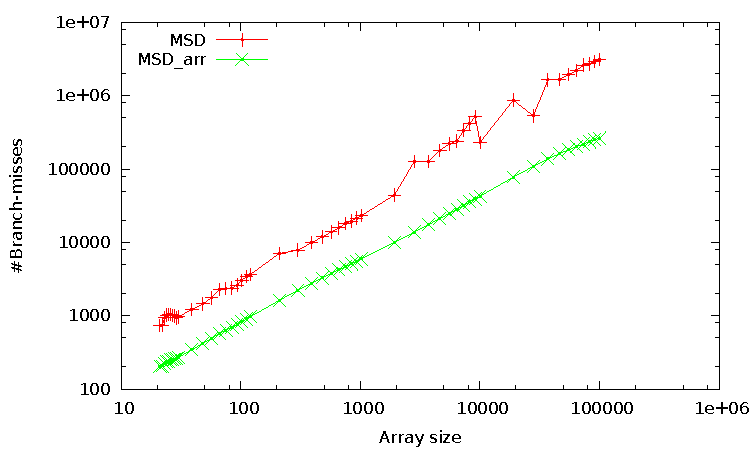
\includegraphics[width=\textwidth]{./Figures/Project2b/Branch_misses.pdf}
		\rule{35em}{0.5pt}
	\caption[Branch misses]{
	Bla bla bla.
	}
	\label{fig:Branch_misses}
\end{figure}


\begin{figure}[htbp]
	\centering
		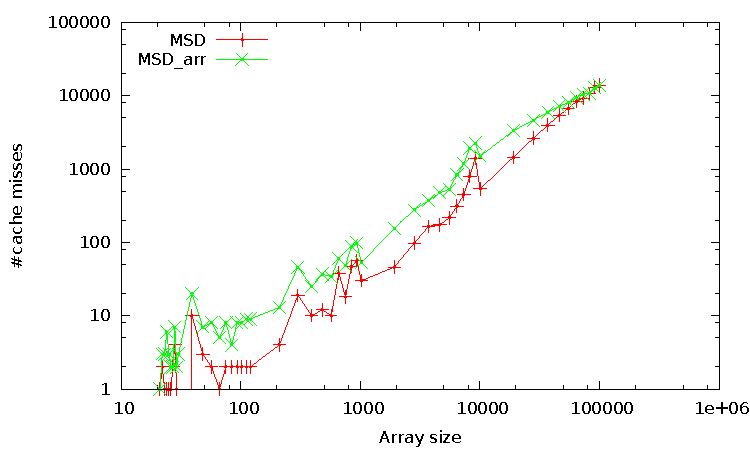
\includegraphics[width=\textwidth]{./Figures/Project2b/Cache_misses.pdf}
		\rule{35em}{0.5pt}
	\caption[Cache misses]{
	Bla bla bla.
	}
	\label{fig:Cache_misses}
\end{figure}



\begin{figure}[htbp]
	\centering
		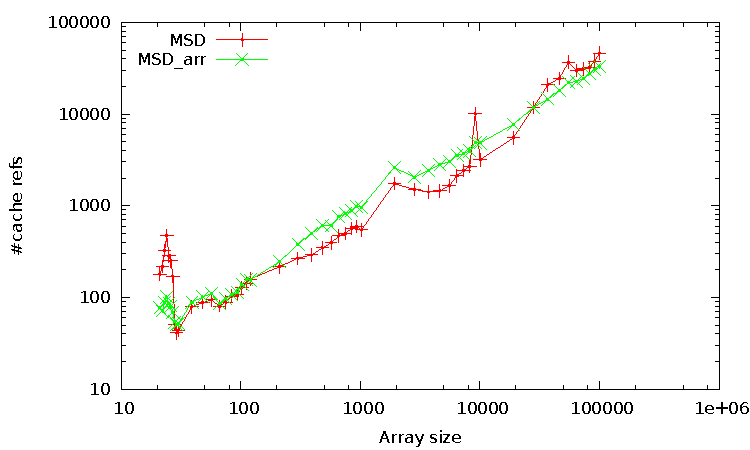
\includegraphics[width=\textwidth]{./Figures/Project2b/Cache_refs.pdf}
		\rule{35em}{0.5pt}
	\caption[Cache refs]{
	Bla bla bla.
	}
	\label{fig:Cache_refs}
\end{figure}



\begin{figure}[htbp]
	\centering
		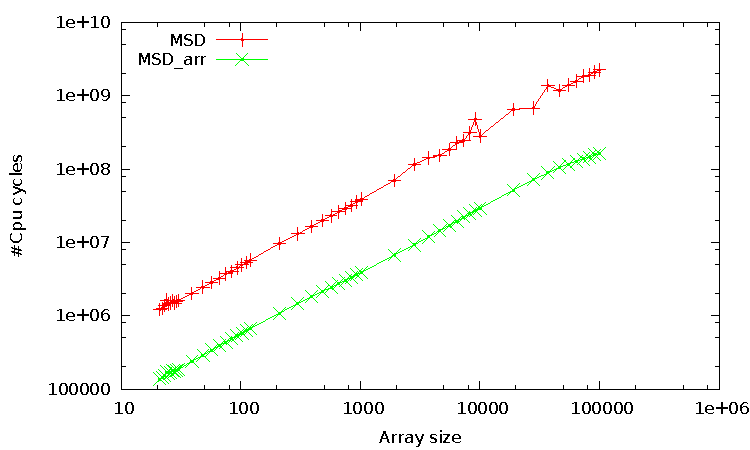
\includegraphics[width=\textwidth]{./Figures/Project2b/Cpu_cycles.pdf}
		\rule{35em}{0.5pt}
	\caption[CPU cycles]{
	Bla bla bla.
	}
	\label{fig:Cpu_cycles}
\end{figure}


\begin{figure}[htbp]
	\centering
		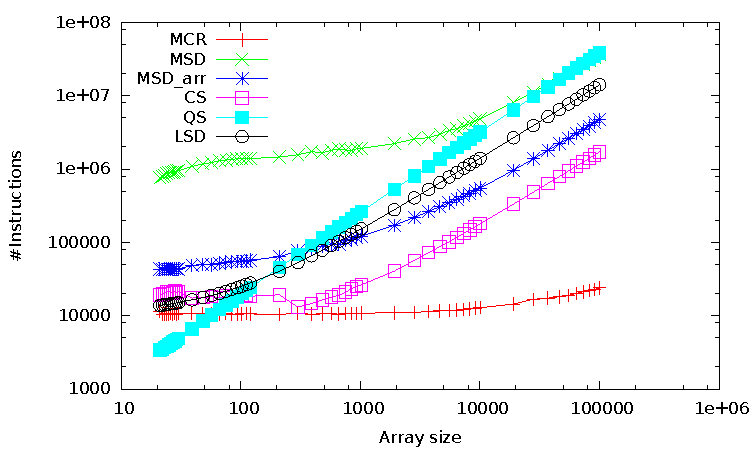
\includegraphics[width=\textwidth]{./Figures/Project2b/Instructions.pdf}
		\rule{35em}{0.5pt}
	\caption[Instructions]{
	Bla bla bla.
	}
	\label{fig:Instructions}
\end{figure}

\begin{figure}[htbp]
	\centering
		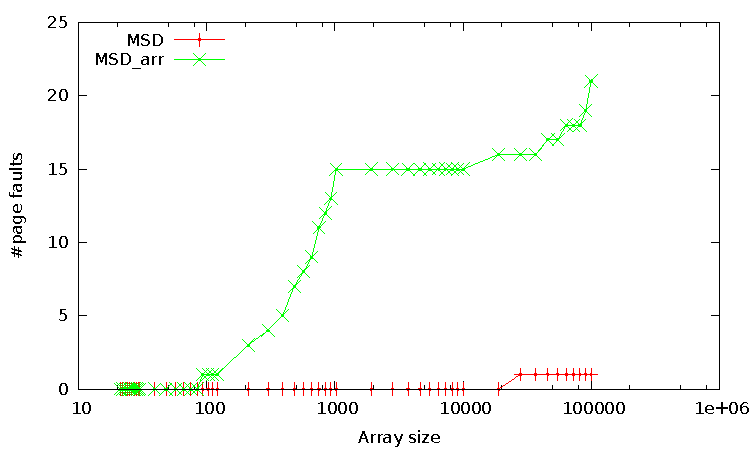
\includegraphics[width=\textwidth]{./Figures/Project2b/Page_faults.pdf}
		\rule{35em}{0.5pt}
	\caption[Page faults]{
	Bla bla bla.
	}
	\label{fig:Page_faults}
\end{figure}


